\documentclass{cekarticle}
\usepackage{color}
\usepackage{amsmath}
\usepackage{amssymb}
\usepackage{array}

\begin{document}

%=============================================================================
% Title page
%=============================================================================

\title{Systems Biology Markup Language (SBML) Level 2 Proposal: Miscellaneous Features}

\author{Andrew Finney, Victoria Gor, Eric Mjolsness, Hamid Bolouri}

\authoremail{
\begin{minipage}{\textwidth}\centering
afinney@cds.caltech.edu, gor@aig.jpl.nasa.gov,\\Eric.D.Mjolsness@jpl.nasa.gov, hbolouri@cds.caltech.edu
\end{minipage}}

\maketitlepage

%=============================================================================
\section{Introduction}
\label{sec:introduction}
%=============================================================================

This document describes proposed features for inclusion in
Systems Biology Markup Language (SBML) Level 2. These features do
not address specific requirements that will enable SBML Level 2
to represent biochemical structures and processes but instead
could potentially form a useful foundation for the features
proposed elsewhere for inclusion in SBML Level 2.

This document is not a definition of SBML Level 2 or part of it.
This document simply presents various features which could be
incorporated into SBML Level 2 as the Systems Biology community
wishes.  This document is intended for detailed review by that
community and to provoke alternative proposals.  Throughout this
document issues that the authors believe will require further
discussion have been highlighted.

The features proposed here are:

\begin{itemize}
\item \textbf{Packages} : a mechanism that enables a model to
document what SBML Level 2 features are used within the model.
see section~\ref{sec:features}.
\item \textbf{Conditional Expressions} : conditional operators
in formulas.  see section~\ref{sec:conditional}.
\item \textbf{Functions} : a mechanism for defining new
functions for use in formulas.  see section~\ref{sec:functions}.
\end{itemize}

Section~\ref{sec:example} includes a complete model which uses
all the features described in this proposal.

For brevity the text of this document is with reference to SBML
Level 1~\citep{hucka:2001} i.e. features are described in terms
of changes to SBML Level 1.  This document uses UML diagrams in
the same way except that new features are shown in red.

All types proposed in this document will be derived from the
\texttt{SBase} type.

\section{Minimal Header for SBML Level 2 documents}

We suggest that the minimal header, that SBML level 2 documents will have, is:

\begin{example}
<?xml version="1.0" encoding="UTF-8"?>
<sbml xmlns="http://www.sbml.org/sbml/level2" version="1" level="2">
\end{example}

\section{Packages}
\label{sec:features}

It is unlikely that systems parsing SBML Level 2 will have
functional internal representations of all the features proposed
for Level 2, for example a given simulator might have a
representation of modularity but not of geometric structures. To
enable a parsing system to check whether a given model is within
its scope it's proposed that an SBML document has an optional
list of \texttt{Package} structures that define the features that
are used by the document.  The proposed new UML definition of the SBML
type is shown in figure~\ref{fig:sbml}.

\begin{figure}[h]
  \vspace*{8pt}
  \centering
  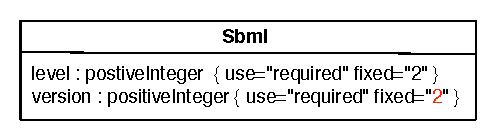
\includegraphics[scale = 0.7]{sbml}
  \caption{The definition of the SBML type}
  \label{fig:sbml}
\end{figure}

In this proposal an \texttt{SBML} structure can optionally
contain a list of \texttt{Features}.  The proposed UML definition of the
\texttt{Feature} type is shown in figure~\ref{fig:feature}.

\begin{figure}[h]
  \vspace*{8pt}
  \centering
  \includegraphics[scale = 0.7]{feature}
  \caption{The definition of the Feature type}
  \label{fig:feature}
\end{figure}

The set of \texttt{Feature} subtypes is very tentative.  It is
proposed that for each of the \texttt{Feature} subtypes there
will be defined a set of SBML elements, numeric expression
functions and numeric expression operators. (These sets will be
defined later).  Each of these sets constitutes a
\emph{package}.  A \emph{package} is used if the document
contains any of the elements or operators in the \emph{package}.

The following proposed list describes the expected scope of each of the
\emph{packages} corresponding to each \texttt{Package} types:
\begin{itemize}
\item \textbf{Geometry}: features needed to support 2D and 3D spatial
models
\item \textbf{Diagrams}: features to store diagrams of models
\item \textbf{Metadata}: features to annotate models, to facilitate
(amongst other things), the linking of model entities to data
external to the models and the systematic storage and retrieval
of models.
\item \textbf{Arrays}: features enabling the inclusion of arrays of
structures/entities in models.  These features would allow a model
to be assembled from many copies of identical parts.  These
features enable the representation of patterns of connection
amongst elements of arrays.
\item \textbf{Multistate}: features enabling the representation of
biochemical entities with a hierarchy of possible states and
applying reactions to those entities with a defined range of
states.  This group is also exploring possible schemes for
representing entities, or complexes, which are graphs of
component entities.
\item \textbf{Modularity}: features enabling the construction of models
from a hierarchy of submodels.  This will allow a given reaction
or process to be modeled at multiple levels of detail.  These
features will allow the construction of models from reusable
components.
\item \textbf{Conditionals}: incorporates conditional operators into
numeric expressions.
\end{itemize}

In this proposal a valid level 2 document would use a subset of
the \emph{packages} that correspond to the \texttt{Package}
elements in the document. The \texttt{Package} lists should not
contain more than one element of a each \texttt{Package} type. An
empty \texttt{Package} list corresponds to the list containing
all possible \texttt{Package} types i.e. the document can contain
any Level 2 operators or elements.  Ideally a document should
contain the smallest non empty valid list of \texttt{Package} structures.

The above list assumes that all systems will be able to support
the functions feature described in section~\ref{sec:functions}.

It is expected that the \texttt{modularity} \emph{package} will allow
more than one \texttt{Model} structure to be contained in an SBML
Level 2 document.  The \texttt{Package} list is a attached to the
\texttt{SBML} structure to ensure that information on the features
used isn't distributed through the document.

\subsection{Example}

The following example of an SBML document header, complying with
this proposal, indicates that the document uses the \texttt{arrays} and
\texttt{conditionals} features.

\begin{example}
<?xml version="1.0" encoding="UTF-8"?>
<sbml xmlns="http://www.sbml.org/sbml/level2" version="1" level="2">
    <listOfFeatures>
        <arrays/>
        <conditionals/>
    </listOfFeatures>
    <model name="cell">
    ...
    </model>
</sbml>
\end{example}

\subsection{Issues}

Some issues that need to be addressed:
\begin{itemize}
\item this concept might be better addressed using separate
namespaces for the different \emph{packages} however this won't
cover the use of operators or functions.  The idea behind this concept is to
enable an event driven parse to halt parsing as soon as the
\texttt{sbml} open tag has been parsed.  As different namespaces
can be added on an ad hoc basis throughout a document, an event
driven parser will have to load the entire document to find all
the namespaces and thus features used in the document.

\item the classification of features will require review at the
end of the development of SBML Level 2.

\item should the \texttt{Conditionals} type be split into
a \texttt{DynamicConditionals} type and a \\
\texttt{StaticConditionals} type? The distinction being between
those conditional expressions where the condition expression
could potentially change during any simulation of the model
(\texttt{DynamicConditionals}) and those that do not
(\texttt{StaticConditionals}).  This information may be an
important criteria by which a simulator will judge whether it can
simulate a model.

\item \texttt{DynamicConditionals} can't be mapped to SBML Level 1.
\end{itemize}

\section{Conditional expressions}
\label{sec:conditional}

This section proposes constructs, for describing discontinuities
via numeric expressions or formula strings.

\subsection{Operators}
Table~\ref{tab:operators} shows a possible extended set of operators that could be
available in SBML Level 2.  New operators are shown in red.  As in
SBML Level 1 these operators work as defined in C except that the
types are always \texttt{double}.  This means that 0 is
interpreted as false and all non zero numbers are interpreted as
true.  The operators \verb|&&| and \verb+||+ short circuit the
evaluation of their second operand depending on the value of the
first operand.

\begin{table}[tbh]
  \vspace*{8pt}
  \begin{center}
    \begin{tabular}{lllcl}
      \toprule
      \textbf{Tokens} & \textbf{Operation} & \textbf{Class} & \textbf{Precedence} & \textbf{Associates} \\
      \midrule
      \emph{name} & symbol reference & operand & 10 & n/a \\
      (\emph{expression}) & expression grouping & operand & 10 & n/a\\
      \emph{f}(\emph{...}) & function call & prefix & 10 & left\\
      \color{red} $!$ & \color{red} logical not & \color{red} unary & \color{red} 9 & \color{red} right\\
      $-$ & negation & unary & 9 & right\\
      \verb|^| & power & binary & 8 & left \\
      $*$ & multiplication & binary & 7 & left\\
      $/$ & division & binary & 7 & left\\
      $+$ & addition & binary & 6 & left\\
      $-$ & subtraction & binary & 6 & left\\
      \color{red} \verb|<| & \color{red} less than & \color{red} binary & \color{red} 5 & \color{red} left\\
      \color{red} \verb|>| & \color{red} greater than & \color{red} binary & \color{red} 5 & \color{red} left\\
      \color{red} \verb|>=| & \color{red} greater than or equal & \color{red} binary & \color{red} 5 & \color{red} left\\
      \color{red} \verb|<=| & \color{red} less than or equal & \color{red} binary & \color{red} 5 & \color{red} left\\
      \color{red} \verb|==| & \color{red} equality & \color{red} binary & \color{red} 4 & \color{red} left\\
      \color{red} \verb|!=| & \color{red} inequality & \color{red} binary & \color{red} 4 & \color{red} left\\
      \color{red} \verb|&&| & \color{red} logical and & \color{red} binary & \color{red} 3 & \color{red} left\\
      \color{red} \verb+||+ & \color{red} logical or & \color{red} binary & \color{red} 2 & \color{red} left \\
      \color{red} \verb|? :| & \color{red} conditional & \color{red} ternary & \color{red} 1 & \color{red} right \color{black} \\
      \bottomrule
    \end{tabular}
  \end{center}
  \caption{A table of the expression operators available in SBML,
    operators proposed in this document are shown in red.  In the
    \textbf{\textrm{Class}} column, ``operand'' implies the construct is an
    operand, ``prefix'' implies the operation is applied to the following
    arguments, ``unary'' implies there is one argument, and ``binary''
    implies there are two arguments.  The values in the
    \textbf{\textrm{Precedence}} column show how the order of different
    types of operation are determined.  For example, the expression $a * b
    + c$ is evaluated as $(a * b) + c$ because the \texttt{*} operator has
    higher precedence.  The \textbf{\textrm{Associates}} column shows how
    the order of similar precedence operations is determined; for example,
    $a - b + c$ is evaluated as $(a - b) + c$ because the $+$ and $-$
    operators are left-associative.  The precedence and associativity rules
    are taken from the C programming language~\protect\citep{harbison:1995},
    except for the symbol \texttt{\^}, which is used in C for a different
    purpose.}
  \label{tab:operators}
\end{table}

\subsection{\texttt{switch} function}

In addition to the new operators described above it is proposed
that an additional `built-in' function \texttt{switch}, is
introduced. This has the form:
\begin{example}
switch(key, match1, result1, ... matchn, resultn, defaultResult);
\end{example}

This function compares \texttt{key} to the values
\texttt{match1...matchn} and returns the \texttt{result} value
immediately following the matching \texttt{match} argument.  If
none of the \texttt{match} arguments are equal to \texttt{key}
then \texttt{switch} returns the \texttt{defaultResult} argument.

The call
\begin{example}
switch(k, m, r, d)
\end{example}
is equivalent to
\begin{example}
(k == m) ? r : d
\end{example}
The call
\begin{example}
switch(k, m1, r1, m2, r2, d)
\end{example}
is equivalent to
\begin{example}
(k == m1) ? r1 : ((k == m2) ? r2 : d)
\end{example}
and so on.

\subsection{Issues}

Given that the function \texttt{switch} and the operators
\texttt{<=}, \texttt{>=} and \texttt{!=} are redundant should
they be incorporated into SBML Level 2?

\section{Functions}
\label{sec:functions}

So as to avoid the continuous revision of SBML, as additional
built-in functions are required, a mechanism is required to allow
the arbitrary definition of new functions in SBML Level 2. This
section proposes such a mechanism.

The proposed UML definition of the \texttt{Model} type is shown in
figure~\ref{fig:model}. (In SBML Level 2 the model type will
probably contain additional optional substructures which are not
shown).  A \texttt{Model} can optionally contain a list of
\texttt{Functions}. Figure~\ref{fig:function} shows the proposed
form of the \texttt{Function} type in UML form.

\begin{figure}[h]
  \vspace*{8pt}
  \centering
  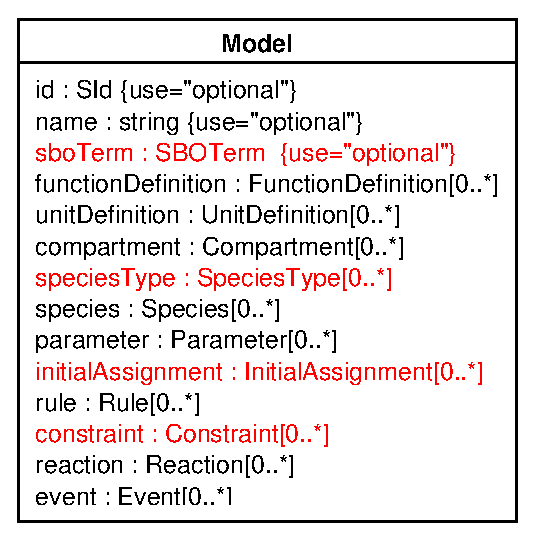
\includegraphics[scale = 0.7]{model}
  \caption{The definition of the Model type}
  \label{fig:model}
\end{figure}

\begin{figure}[h]
  \vspace*{8pt}
  \centering
  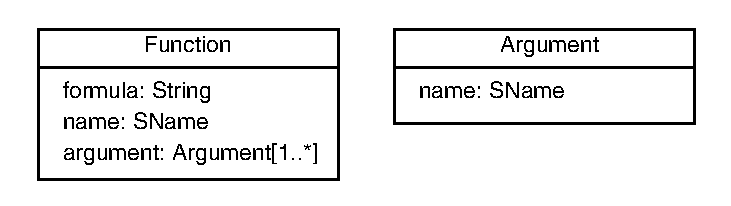
\includegraphics[scale = 0.7]{function}
  \caption{The definition of the Function type}
  \label{fig:function}
\end{figure}

A proposed \texttt{Function} structure consists of the function's name (of
\texttt{SName} type), a formula string and a list of
\texttt{Argument} structures. An \texttt{Argument} structure
simply consists of the argument's name.

A proposed \texttt{Function} structure defines a new function that can be
used in any formula that follows the \texttt{Function} structure.
The only symbols that can be used in the formula string of a
\texttt{Function} structure are the following:
\begin{itemize}
\item \textbf{Arguments:} any of the names given in the \texttt{Argument} list.
\item \textbf{Previously defined functions:} any of the names given in preceding \texttt{Function} structures.
\item \textbf{Built-in functions:} any of the names of built-in functions.
\end{itemize}
These restrictions mean that functions can't be recursive or
mutually recursive thus ensuring that function `calls' can be
expanded in place i.e. models using functions can be mapped to
SBML Level 1.

A \texttt{Function} formula simply returns a \texttt{double}
value.  All the arguments to a function are of type
\texttt{double}.  These functions share the same namespace as
other model-level components, this means that, for example a
function can't have the same name as a specie or a reserved name.

\subsection{Example}

The following is a simple example of a \texttt{Function}
structure in a \texttt{Model} structure:

\begin{example}
<model name="cell">
    <listOfFunctions>
        <function name="pow3" formula="x^3">
            <listOfArguments>
                <argument name="x"/>
            </listOfArguments>
        </function>
    </listOfFunctions>
    ...
</model>
\end{example}

\subsection{Issues}
\begin{itemize}
\item Is the scope of symbols in formulas in functions too restrictive?
\item Do we need to be able to handle objects other than \texttt{double} values?
\end{itemize}

\section{Models with no reactions}

It is proposed that in SBML Level 2 a model can contain no
reactions.  A \texttt{specieConcentrationRule} structures can be
defined to have the same effect as reactions.

\section{Complete Example}
\label{sec:example}

This section contains a complete SBML document which
includes all the proposed features described here.  This model is a
variation on the example model described in~\citet{hucka:2001}.

Consider the following hypothetical branched system:
\begin{equation*}
  \begin{array}{@{}ccc@{}}
    X_0 & \underrightarrow{k_1 pow3(X_0)} & S_1 \\ \\[-4pt]
    S_1 & \underrightarrow{\text{if $S_1 < 1$ then $k_a S_1$ else $k_b S_2$}} & X_1 \\ \\[-4pt]
    S_1 & \underrightarrow{k_3 S_1} & X_2
  \end{array}
\end{equation*}

The following is a XML document that encodes the model shown
above:
\begin{example}
<?xml version="1.0" encoding="UTF-8"?>
<sbml xmlns="http://www.sbml.org/sbml/level2" version="1" level="2">
    <listOfFeatures>
        <conditionals/>
    </listOfFeatures>
    <model name="Branch">
        <notes>
            <body xmlns="http://www.w3.org/1999/xhtml">
                <p>Simple branch system.</p>
                <p>The reaction looks like this:</p>
                <p>reaction-1:   X0 -> S1; k1* pow3(X0);</p>
                <p>reaction-2:   S1 -> X1; S1 < 1 ? k2a*S1 : k2b*S2 ;</p>
                <p>reaction-3:   S1 -> X2; k3*S1;</p>
                <p>where pow3(x) is x^3
            </body>
        </notes>
        <listOfFunctions>
            <function name="pow3" formula="x^3">
                <listOfArguments>
                    <argument name="x"/>
                </listOfArguments>
            </function>
        </listOfFunctions>
        <listOfCompartments>
            <compartment name="compartmentOne" volume="1"/>
        </listOfCompartments>
        <listOfSpecies>
            <specie name="S1" initialAmount="0" compartment="compartmentOne"
                    boundaryCondition="false"/>
            <specie name="X0" initialAmount="0" compartment="compartmentOne"
                    boundaryCondition="true"/>
            <specie name="X1" initialAmount="0" compartment="compartmentOne"
                    boundaryCondition="true"/>
            <specie name="X2" initialAmount="0" compartment="compartmentOne"
                    boundaryCondition="true"/>
        </listOfSpecies>
        <listOfReactions>
            <reaction name="reaction_1" reversible="false">
                <listOfReactants>
                    <specieReference specie="X0" stoichiometry="1"/>
                </listOfReactants>
                <listOfProducts>
                    <specieReference specie="S1" stoichiometry="1"/>
                </listOfProducts>
                <kineticLaw formula="k1 * pow3(X0)">
                    <listOfParameters>
                        <parameter name="k1" value="0"/>
                    </listOfParameters>
                </kineticLaw>
            </reaction>
            <reaction name="reaction_2" reversible="false">
                <listOfReactants>
                    <specieReference specie="S1" stoichiometry="1"/>
                </listOfReactants>
                <listOfProducts>
                    <specieReference specie="X1" stoichiometry="1"/>
                </listOfProducts>
                <kineticLaw formula="S1 < 1 ? ka*S1 : kb*S2">
                    <listOfParameters>
                        <parameter name="ka" value="0"/>
                        <parameter name="kb" value="1"/>
                    </listOfParameters>
                </kineticLaw>
            </reaction>
            <reaction name="reaction_3" reversible="false">
                <listOfReactants>
                    <specieReference specie="S1" stoichiometry="1"/>
                </listOfReactants>
                <listOfProducts>
                    <specieReference specie="X2" stoichiometry="1"/>
                </listOfProducts>
                <kineticLaw formula="k3 * S1">
                    <listOfParameters>
                        <parameter name="k3" value="0"/>
                    </listOfParameters>
                </kineticLaw>
            </reaction>
        </listOfReactions>
    </model>
</sbml>
\end{example}

%=============================================================================
% References
%=============================================================================

\bibliographystyle{apalike}
\bibliography{strings,a,b,c,d,e,f,g,h,i,j,k,l,m,n,o,p,q,r,s,t,u,v,w,x,y,z}
\end{document}
